\documentclass[tikz]{standalone}
\usepackage{pgfplots}
\pgfplotsset{compat=1.15}
\usepackage{mathrsfs}
\usetikzlibrary{arrows,calc}
\usepackage{tkz-euclide}

\usepackage{fp}
\pagestyle{empty}

\definecolor{AngleClr}{rgb}{0,0.39215686274509803,0}
\definecolor{ShapeClr}{rgb}{0.6,0.2,0}

\begin{document}

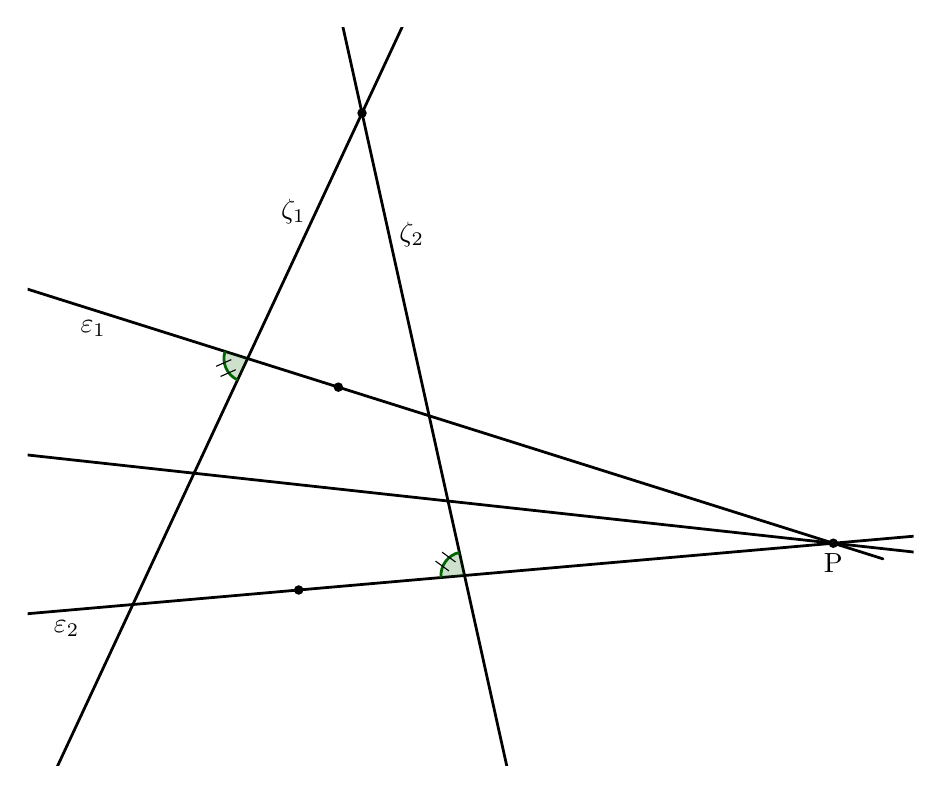
\begin{tikzpicture}[scale=.75]

\clip(-4.5,-4) rectangle (10.5,8.5);

\tkzSetUpLine[line width=1pt,color=black]
\tkzSetUpPoint[fill=black]

\tkzDefPoint(105:3){A}
\tkzDefPoint(-155:3){B}
\tkzDefPoint(-15:3){C}
\tkzDefPoint(40:3){D}

\tkzDefTriangleCenter[circum](A,B,C) \tkzGetPoint{O}

\tkzInterLL(A,B)(C,D) \tkzGetPoint{I1}
\tkzInterLL(A,D)(B,C) \tkzGetPoint{I2}

\tkzDefLine[bisector](A,I2,B) \tkzGetPoint{x}
\tkzInterLL(I2,x)(A,B) \tkzGetPoint{K1}
\tkzInterLL(I2,x)(C,D) \tkzGetPoint{K2}

\tkzDrawSegments[add=2.5 and 2.5](A,B C,D A,D B,C I2,K2)



\tkzDefPointOnLine[pos=-0.4](A,D)\tkzGetPoint{E}
\tkzDefPointOnLine[pos=0.5](A,D)\tkzGetPoint{M1}
\tkzDefPointOnLine[pos=0.5](B,C)\tkzGetPoint{M2}

\tkzFillAngles[fill=AngleClr,size=.4,fill opacity=0.2](D,C,B E,A,B)
\tkzMarkAngles[line width=1pt,size=.4,color=AngleClr,mark=||,mksize=3](D,C,B E,A,B)

\tkzDrawPoints[size=3](M1,M2,I1,I2)

\tkzLabelPoint[below](I2){$\rm P$}

\tkzLabelSegment[pos=-0.85](A,D){$\varepsilon_1$}
\tkzLabelSegment[pos=-0.2](B,C){$\varepsilon_2$}

\tkzLabelSegment[pos=0.4,left](I1,A){$\zeta_1$}
\tkzLabelSegment[pos=0.4,right](I1,D){$\zeta_2$}
\end{tikzpicture}

\end{document}
